\chapter{Presentación de los datos, Análisis, Discusión}

En algunas disciplinas, el capítulo Presentación de datos va acompañado del análisis o de la discusión de la información (\textit{Presentación y análisis de los datos}; \textit{Resultados y discusión}), en tanto que en otras, \textit{Presentación}, \textit{Análisis} y \textit{Discusión} son capítulos separados.
El objetivo de esta(s) parte(s) de la tesis es presentar los datos recabados y el análisis realizado a la luz de la bibliografía ya revisada. Se puede incluir la interpretación de los resultados (\textit{Discusión}) a partir del análisis de los datos, o también relacionarlos con estudios relevantes que se entienden pertinentes, aun si estos no se han consignado en los \textit{Fundamentos teóricos}, ya que se entiende que al analizar los datos pueden aparecer algunos que no se enmarcan teóricamente o que no se explican en el encuadre teórico o en estudios ya existentes.

Ahora a modo de ejemplo mencionamos el símbolo de los números reales utilizando el comando \verb|\gls{}| \gls{Real} y el comando \verb|\glssymbol{}| \glssymbol{Real}. Otro ejemplo es mencionar el tensor simétrico de tensiones \gls{sigma}, o un valor escalar  \gls{alph} o un conjunto vacío \gls{emptyset}.

También se encuentra la posibilidad de realizar un control de cambios de la tesis, de manera muy simple. En este caso se soporta hasta tres correctores distintos, cuyas iniciales se declaran al inicio con un color distinto asignado. En este caso se tiene los correctores \textcolor{redtex}{JLM}, \textcolor{bluetex}{JH} y \textcolor{greentex}{MC}. Los correctores deberían de recibir el archivo \verb|tesis.tex|, con todos los archivos dependientes de este para poder hacer los cambios y compilar la tesis. 

Este es un ejemplo en donde se puede sugerir agregar texto \added[id=JLM,remark={a este}]{documento}. Otra \added[id=JLM,remark={Acá hay un ejemplo de un texto bastante largo que se agrega como cambio}]{manera} de utilizar el control de cambios sería la de \deleted[id=JH]{agregar} eliminar texto. También se podría utilizar la funcionalidad de agregar notas referidas a cierta oración o temática. \note[id=JH]{Muy buen análisis!}. Por último se encuentra la opción de reemplazar cierto texto por otro \replaced[id=MC]{poner esta oración.}{Mejor quitemos esto.}

\section{Título de sección}

Ejemplo de tabla

\begin{table}[h!]
\centering
\caption{Leyenda de tabla.}
\label{tab:comp}
\begin{tabular}{|c|c|c|}
  \hline
  $t$ (seg) & $x$(t) & $y$(t)\\
  \hline
  1 & 0.0000 & 0.0001\\
  2 & 0.5000 & 0.2498\\
  3 & 1.0000 & 1.0000\\
  4 & 1.5000 & 2.2403\\
  5 & 2.0000 & 4.0010\\
  6 & 2.5000 & 6.2459\\
  \hline
\end{tabular}
\end{table}

Ejemplo de figura.

\begin{figure}[h!]
\label{fig:comp}
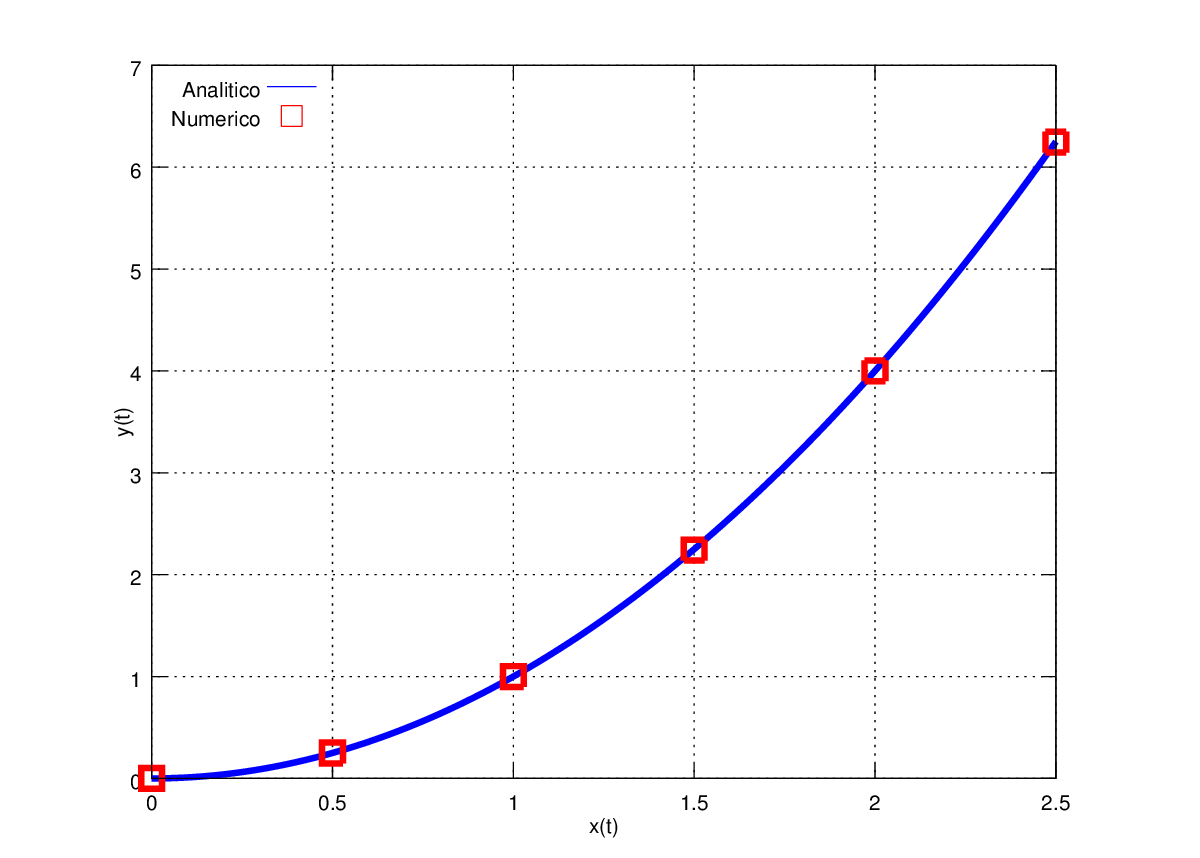
\includegraphics[width=.8\textwidth]{imagenes/chap4/x_vs_y}
\caption{Leyenda de figura.}
\end{figure}
Ejemplo de ecuación:
\begin{equation}
y(x)=x^2
\end{equation}
